%%%%%%%%%%%%%%%%%%%%%%%%%%%%%%%%%%%%%%%%%
% Masters Thesis 
% LaTeX Template
%
% This template is based on a template by:
% Steve Gunn (http://users.ecs.soton.ac.uk/srg/softwaretools/document/templates/)
% Sunil Patel (http://www.sunilpatel.co.uk/thesis-template/)
%
% Template license:
% CC BY-NC-SA 3.0 (http://creativecommons.org/licenses/by-nc-sa/3.0/)
%
%%%%%%%%%%%%%%%%%%%%%%%%%%%%%%%%%%%%%%%%%

%----------------------------------------------------------------------------------------
%	PACKAGES AND OTHER DOCUMENT CONFIGURATIONS
%----------------------------------------------------------------------------------------

\documentclass[
11pt, % The default document font size, options: 10pt, 11pt, 12pt
%oneside, % Two side (alternating margins) for binding by default, uncomment to switch to one side
english, % ngerman for German
singlespacing, % Single line spacing, alternatives: onehalfspacing or doublespacing
%draft, % Uncomment to enable draft mode (no pictures, no links, overfull hboxes indicated)
%nolistspacing, % If the document is onehalfspacing or doublespacing, uncomment this to set spacing in lists to single
%liststotoc, % Uncomment to add the list of figures/tables/etc to the table of contents
%toctotoc, % Uncomment to add the main table of contents to the table of contents
%parskip, % Uncomment to add space between paragraphs
%nohyperref, % Uncomment to not load the hyperref package
headsepline, % Uncomment to get a line under the header
%chapterinoneline, % Uncomment to place the chapter title next to the number on one line
%consistentlayout, % Uncomment to change the layout of the declaration, abstract and acknowledgements pages to match the default layout
]{MastersDoctoralThesis} % The class file specifying the document structure

\usepackage[utf8]{inputenc} % Required for inputting international characters
\usepackage[T1]{fontenc} % Output font encoding for international characters

\usepackage{mathpazo} % Use the Palatino font by default

\usepackage[backend=bibtex,style=authoryear,natbib=true]{biblatex} % Use the bibtex backend with the authoryear citation style (which resembles APA)

\addbibresource{example.bib} % The filename of the bibliography

\usepackage[autostyle=true]{csquotes} % Required to generate language-dependent quotes in the bibliography

% Extra packages
\usepackage[inline]{enumitem}
\usepackage{amsmath}
\usepackage{float}
\usepackage{amsmath}
\usepackage{tablefootnote}
\usepackage{algorithm}
\usepackage{algpseudocode}

\DeclareMathOperator*{\argmin}{\arg\!\min}
%----------------------------------------------------------------------------------------
%	MARGIN SETTINGS
%----------------------------------------------------------------------------------------

\geometry{
	paper=a4paper, % Change to letterpaper for US letter
	inner=2.5cm, % Inner margin
	outer=3.8cm, % Outer margin
	bindingoffset=.5cm, % Binding offset
	top=1.5cm, % Top margin
	bottom=1.5cm, % Bottom margin
	%showframe, % Uncomment to show how the type block is set on the page
}

%----------------------------------------------------------------------------------------
%	THESIS INFORMATION
%----------------------------------------------------------------------------------------

\thesistitle{Learning with invariants} % Your thesis title, this is used in the title and abstract, print it elsewhere with \ttitle
\supervisor{Dr. Oriol \textsc{Pujol}} % Your supervisor's name, this is used in the title page, print it elsewhere with \supname
\examiner{} % Your examiner's name, this is not currently used anywhere in the template, print it elsewhere with \examname
\degree{MSc} % Your degree name, this is used in the title page and abstract, print it elsewhere with \degreename
\author{Vladislav \textsc{Nikolov}} % Your name, this is used in the title page and abstract, print it elsewhere with \authorname
\addresses{} % Your address, this is not currently used anywhere in the template, print it elsewhere with \addressname

\subject{Computer Science} % Your subject area, this is not currently used anywhere in the template, print it elsewhere with \subjectname
\keywords{} % Keywords for your thesis, this is not currently used anywhere in the template, print it elsewhere with \keywordnames
\university{\href{http://www.ub.edu}{Universitat de Barcelona}} % Your university's name and URL, this is used in the title page and abstract, print it elsewhere with \univname
\department{\href{http://department.university.com}{}} % Your department's name and URL, this is used in the title page and abstract, print it elsewhere with \deptname
\group{\href{http://researchgroup.university.com}{}} % Your research group's name and URL, this is used in the title page, print it elsewhere with \groupname
\faculty{\href{http://mat.ub.edu}{Facultat de Matemàtiques i Informàtica}} % Your faculty's name and URL, this is used in the title page and abstract, print it elsewhere with \facname

\AtBeginDocument{
\hypersetup{pdftitle=\ttitle} % Set the PDF's title to your title
\hypersetup{pdfauthor=\authorname} % Set the PDF's author to your name
\hypersetup{pdfkeywords=\keywordnames} % Set the PDF's keywords to your keywords
}

\begin{document}

\frontmatter % Use roman page numbering style (i, ii, iii, iv...) for the pre-content pages

\pagestyle{plain} % Default to the plain heading style until the thesis style is called for the body content

%----------------------------------------------------------------------------------------
%	TITLE PAGE
%----------------------------------------------------------------------------------------

\begin{titlepage}
\begin{center}

\vspace*{.06\textheight}
{\scshape\LARGE \univname\par}\vspace{1.5cm} % University name
\textsc{\Large Fundamental Principles of Data Science Master's Thesis}\\[0.5cm] % Thesis type

\HRule \\[0.4cm] % Horizontal line
{\huge \bfseries \ttitle\par}\vspace{0.4cm} % Thesis title
\HRule \\[1.5cm] % Horizontal line
 
\begin{minipage}[t]{0.4\textwidth}
\begin{flushleft} \large
\emph{Author:}\\
\href{http://www.johnsmith.com}{\authorname} % Author name - remove the \href bracket to remove the link
\end{flushleft}
\end{minipage}
\begin{minipage}[t]{0.4\textwidth}
\begin{flushright} \large
\emph{Supervisor:} \\
\href{http://www.jamessmith.com}{\supname} % Supervisor name - remove the \href bracket to remove the link  
\end{flushright}
\end{minipage}\\[3cm]
 
\vfill

\large \textit{A thesis submitted in partial fulfillment of the requirements\\ for the degree of MSc in Fundamental Principles of Data Science}\\[0.3cm] % University requirement text
\textit{in the}\\[0.4cm]
\facname\\[2cm] % Research group name and department name
 
\vfill

{\large \today}\\[4cm] % Date
%\includegraphics{Logo} % University/department logo - uncomment to place it
 
\vfill
\end{center}
\end{titlepage}


%----------------------------------------------------------------------------------------
%	ABSTRACT PAGE
%----------------------------------------------------------------------------------------

\begin{abstract}
\addchaptertocentry{\abstractname} % Add the abstract to the table of contents
The Thesis Abstract is written here (and usually kept to just this page). The page is kept centered vertically so can expand into the blank space above the title too\ldots
\end{abstract}

%----------------------------------------------------------------------------------------
%	ACKNOWLEDGEMENTS
%----------------------------------------------------------------------------------------

\begin{acknowledgements}
\addchaptertocentry{\acknowledgementname} % Add the acknowledgements to the table of contents
The acknowledgments and the people to thank go here, don't forget to include your project advisor\ldots
\end{acknowledgements}



%----------------------------------------------------------------------------------------
%	THESIS CONTENT - CHAPTERS
%----------------------------------------------------------------------------------------

\mainmatter % Begin numeric (1,2,3...) page numbering

\pagestyle{thesis} % Return the page headers back to the "thesis" style

\tableofcontents

% Include the chapters of the thesis as separate files from the Chapters folder
% Uncomment the lines as you write the chapters

% Chapter Template

\chapter{Introduction}

\label{Chapter1}

%----------------------------------------------------------------------------------------
%	SECTION 1: MOTIVATION AND BRIEF DESCRIPTION OF THE PROJECT
%----------------------------------------------------------------------------------------

\section{Motivation and brief description of the project}

The current machine learning paradigms consider no further information apart from the data
samples when trying to learn a model that can represent the data and be used later on
to infer information about new samples. During the training process, the current methods
try to minimize the error with respect to the original data, thus searching the function
that best fits the data in an infinite space of functions. However, the training data has
statistical information that can help reduce the searching space to a region of it, allowing
also to find functions that better fit the data.

A new learning paradigm that takes into account the statistical information of the training data
in the form of statistical invariants has been recently proposed by \cite{Vapnik2019}. Thanks to it,
statistical information of the problem can be used in the learning process, which might
be overlooked by most of the models because some relationships between variables are hard to
spot or require prior knowledge that the model does not have access to. Nonetheless,
it seems that this learning paradigm has not been fully explored or applied that much in practice.

Therefore, in this work we would like to further explore the possible applications of this
paradigm and whether it can be made more general, without requiring prior knowledge of the problem.

%----------------------------------------------------------------------------------------
%	SECTION 2: GOALS AND OBJECTIVES
%----------------------------------------------------------------------------------------

\section{Goals and objectives}

In this thesis we aim to
\begin{enumerate*}[label=(\roman*)]
    \item understand and further explore the application of the invariants in the learning
    problem,
    \item propose new invariants that require no previous knowledge of the problem and
    thus can be applied to multiple domains,
    \item automatize the selection process of the most suitable invariants for a new problem and
    \item extend the learning paradigm so that it can be applied to multiclass classification problems.
\end{enumerate*}

In order to accomplish these goals, we propose a series of milestones that must be achieved
first:

\begin{enumerate}
    \item Understand the original paper and reproduce it, which implies implementing the proposed
    algorithms for learning with statistical invariants and reproducing some of the experiments
    and results. Because there is no source code available, we have to start from scratch.
    \item Propose new invariants and apply them to the same problems as the ones in the paper
    to get an initial idea of how they work.
    \item Build a wrapper around the previously defined binary classifier to enable its use
    in multiclass classification problems.
    \item Experiment with multiclass classification problems to test the proposed invariants and
    compare them to a baseline to see whether they are actually helping or not during the learning
    process.
\end{enumerate}

The expected outcome of this work is a small software package that contains a machine learning
model that can be applied to classification problems.

%----------------------------------------------------------------------------------------
%	SECTION 3: BRIEF SUMMARY OF THE RESULTS
%----------------------------------------------------------------------------------------

\section{Brief summary of the results}

With the completion of this work, we have been able to achieve the following objectives:

\begin{itemize}
    \item We have proposed new invariants that can be applied to different problems
    with no prior knowledge required.
    \item We have extended the LUSI paradigm to work with multiclass problems.
    \item We have created a small software module containing the extended version of LUSI as
    a machine learning model. This model has the same interface as a machine learning model
    from \texttt{scikit-learn}, which makes it fully compatible with the functionality provided
    by this module.
\end{itemize}

However, we have also noted that we did not have that much of a success in the following aspects:

\begin{itemize}
    \item We were not able to automatize the selection process of the most suitable invariants
    for a problem. Thus, it still remains an open question.
    \item As we will see in later chapters, the invariants that we have proposed have not achieved
    the best results. The random projections were able to achieve similar but slightly worse results
    compared to the original invariants, and the random hyperplanes seem to provide little to no
    relevant information.
\end{itemize}

Nevertheless, we have been able to better understand the learning with invariants problem
and made some contributions on the topic. All of the developed code and experiments can be
found in this \href{https://github.com/Vol0kin/LUSI}{GitHub repository}.


%----------------------------------------------------------------------------------------
%	SECTION 4: LAYOUT
%----------------------------------------------------------------------------------------

\section{Layout}

This thesis is structured as follows:

\begin{itemize}
    \item Chapter \ref{Chapter1} introduces this work, presenting the main goals that are expected
    to be achieved by the end of it and briefly discussing the obtained results.
    \item Chapter \ref{Chapter2} explains the background work that has inspired this project,
    showing its main contributions and results.
    \item Chapter \ref{Chapter3} proposes a series of invariants that aim to be more general and easy
    to apply to different problems and a method to expand this paradigm to multiclass classification
    problems.
    \item Chapter \ref{Chapter4} studies how the proposed invariants and methods work in practice
    and what results can be achieved with them.
    \item Chapter \ref{Chapter5} briefly discusses what conclusions can be drawn from this work
    and what future work can be done on the topic.
\end{itemize}


% Chapter Template

\newcommand{\Tau}{\mathcal{T}}
\newcommand{\norm}[1]{\lVert #1 \rVert}
\newcommand{\innerprod}[1]{\left< #1 \right>}
\newcommand{\set}[1]{\lbrace #1 \rbrace}

\chapter{Learning using statistical invariants} % Main chapter title
\label{Chapter2}

Given that this work intends to explore the applications of the invariants in the learning
process, we first need to introduce the background work that proposed this new learning
paradigm, which is called LUSI (Learning Using Statistical Invariants).

This chapter intends to provide the necessary background to understand the basis of this work
and an overview of the most relevant aspects of the original paper that presented the LUSI paradigm,
which was proposed by \cite{Vapnik2019}. For further information and more details, please
refer to the original paper.

\section{Weak convergence and the LUSI paradigm}

Supervised machine learning algorithms try to find the best estimate of some conditional probability
function $P(y | x)$, i.e., given a data point $x$, we want to compute the probability that this
point belongs to a particular class $y$.

Classical methods do this by using the strong mode of convergence in the Hilbert space. However,
in the LUSI paradigm this estimation is obtained using the weak mode of convergence. Hence, it is
important to understand the difference between this two modes of convergence and what role
the weak mode of convergence plays in the LUSI paradigm.

\subsection{Strong and weak modes of convergence}

In a Hilbert space, the relationships between two functions $f_1(x)$ and $f_2(x)$ have two
numerical properties:

\begin{enumerate}
    \item The distance between functions
    
    \[
        \rho (f_1, f_2) = \norm{f_1(x) - f_2(x)}
    \]
    
    that is defined by the metric of the $L_2$ space and
    
    \item The inner product between functions
    
    \[
        R(f_1, f_2) = \innerprod{f_1(x), f_2(x)}
    \]
    
    that has to satisfy the corresponding requirements.
\end{enumerate}

These two properties imply two different modes of convergence: a strong one and a weak one. Classical
learning paradigms rely on the strong convergence mode (convergence in metrics), trying to find a
sequence of functions $\set{P_l(y=1 | x)}$\footnote{We focus here in the binary problem setting, i.e. $y\in \{0,1\}$. Thus, $P_l(y=1 | x)$ fully specifies the output probability distribution.} such that

\[
    \lim_{l \to \infty} \norm{P_l(y=1 | x) - P(y=1 | x)} = 0\quad \forall x
\]

The weak mode of convergence (convergence in inner products) is given by

\[
    \lim_{l \to \infty} \innerprod{P_l(y=1 | x) - P(y=1 | x), \psi(x)} = 0\quad \forall \psi(x) \in L_2
\]

Note that this mode of convergence has to take place for \emph{all} functions in the Hilbert space $L_2$.

It is known that the strong mode of convergence implies the weak one, although generally speaking, the
reverse is not true.

\subsection{The LUSI paradigm}

Opposite to the classical learning paradigms, LUSI is based on the weak mode of convergence. It replaces
the infinite set of functions with a set of functions $\mathcal{P} = \set{\psi_1(x), \dots, \psi_m(x)}$
called predicates, which describe some important properties of the desired conditional probability function and
restrict the scope of weak convergence only to the set of functions $\mathcal{P}$. These properties are
called invariants, and can be expressed as the following equalities:

\[
    \int \psi_s P(y=1 | x)dP(x) = \int \psi_s dP(y=1, x) = a_s,\quad s = 1, \dots, m
\]

where $a_s$ is the expected value of the predicate $\psi_s(x)$ with respect to measure
$P(y=1, x)$. These values are unknown but can be estimated using the training data
$\set{(x_i, y_i),\ i = 1, \dots, l}$. Therefore, the previous expression can be rewritten
as follows:

\begin{equation}
    \label{eq:invariant_approximation}
    \frac{1}{l} \sum_{i=1}^l \psi_s(x_i)P_l(y=1 | x_i) \approx a_s \approx \frac{1}{l} \sum_{i=1}^l y_i \psi_s(x_i),\quad
    s = 1, \dots, m
\end{equation}

Simply put, the general idea of the LUSI paradigm is to find an approximation $P_l(y=1|x)$ of the
real conditional probability function in the subset of functions that preserve the invariants
associated to the set of predicates $\mathcal{P}$, reducing effectively the set of candidate functions
to those that satisfy \eqref{eq:invariant_approximation}.

\subsection{Predicate selection}

In order to find this approximation of the conditional probability function, there must exist
some kind of mechanism that allows us to determine which invariants should be used. Luckily,
the authors propose a very simple way to sequentially selecting invariants. Given an approximation
$P_l^m(y=1|x)$ using $m$ invariants and a new predicate $\psi_{m+1}$ which we would to know whether
it should be considered or not. We can compute the following value before adding it:

\begin{equation}
    \label{eq:predicate_selection}
    \Tau = \frac{\left| \sum_{i=1}^l \psi_{m+1}(x_i) P^m_l(y = 1 | x_i) - \sum_{i=1}^l y_i \psi_{m+1}(x_i) \right|}{\sum_{i=1}^l y_i \psi_{m+1}(x_i)}
\end{equation}

If $\Tau \geq \delta$ for some small threshold $\delta$, the new invariant defined by predicate $\psi_{m+1}$
is considered. Otherwise, the expression \eqref{eq:invariant_approximation} is treated as an equality
and the invariant is not considered in the approximation.


\section{Statistical invariants}

A \emph{statistical invariant} is a specific realization of a predicate with statistical meaning.
This means that it captures some sort of statistical information of the data that has to be
conserved when selecting the best approximation of the conditional probability function.

There are different types of statistical invariants, each one of them
providing different information about the data. In this case, the authors have considered
two in particular: the zeroth order and first order moments of the conditional probability
function $P(y=1|x)$. We will briefly discuss each one of them and see what kind of information
they provide.

\subsection{Zeroth order invariant}

Suppose that we are given a binary classification problem, in which the positive instances
are labeled as 1 and the negative ones as 0. The zeroth order invariant would give us information
about the ratio of elements of the positive class. It is defined as follows:

\[
    \psi_{z.o.}(x) = 1
\]

The logic behind it is the following: the predicate is applied to each single sample in the dataset,
which will yield the vector $(1, \dots, 1) \in \mathbb{R}^l $, where $l$ is the number of samples. Taking into account
expression \eqref{eq:invariant_approximation}, we can see that each element of this vector is multiplied
by the predicted labels (left side) and the true labels (right side). These values are summed and then divided
by $l$, which gives us the proportion of positive predicted elements on the left side and the proportion
of true positive elements on the right side. Notice that the invariant is only taken into account for those
elements whose predicted or true label is positive. Thus, the negative samples are not considered.

\subsection{First order invariant}

Suppose the same case scenario as in the previous subsection. If we apply the first order invariant to
a dataset, we would get the mean or centroid of the positive class. Its mathematical expression is:

\[
    \psi_{f.o.}(x) = x
\]

Same as before, when this predicate is applied to the dataset it will generate the vector
$(x_1, \dots, x_l) \in \mathbb{R}^l$. Following expression \eqref{eq:invariant_approximation} again,
only the positive true or predicted elements will be considered. Therefore, their values will be summed and
then averaged, yielding indeed the centroid of the positive class (both for the predicted and true labels).

\section{Solving the learning problem}
\label{sect:solvin_learning_problem}

The authors show that in a specific type of Hilbert space called Reproducing Kernel Hilbert Space (RKHS)
the estimate of the conditional probability function can be computed as

\[
    f(x) = A^T \mathcal{K}(x) + c
\]

where $A \in \mathbb{R}^l$ is a vector of coefficients, $\mathcal{K}(x) = (K(x_1, x), \dots, K(x_l, x))^T$
is a vector of functions determined by the kernel associated to the RKHS\footnote{In this case, the authors have
considered the Gaussian Kernel, which is defined as
\[
    K(x, x') = \exp \lbrace -\delta \norm{x - x'}^2 \rbrace,\; \delta > 0
\]
}
and evaluated on the training data, and $c \in \mathbb{R}$ is the bias term.

Additionally, let $Y = (y_1, \dots, y_l)$  be the labels of the training set,  $K \in \mathbb{R}^{l \times l}$
the matrix with elements $K(x_i, x_j),\; i, j = 1, \dots, l$, $\Phi_s = (\psi_s(x_1), \dots, \psi_s(x_l))^T$
the vector obtained from evaluating the $l$ points of the sample using predicate $\psi_s$,
$1_l = (1, \dots, 1) \in \mathbb{R}^l$ a vector of ones and $V \in \mathbb{R}^{l \times l}$ a matrix called
the $V$-matrix, proposed by \cite{Vapnik2015}, which captures some geometric properties of the data\footnote{The
most simple case considers that the $V$-matrix is equivalent to the identity matrix. Also, the authors found
that using the $V$-matrix over the identity matrix didn't improve the results that much, but it was rather the
use of invariants that made the difference. For the sake of consistency, we are going to keep the $V$-matrix in
the expressions as this is how they are supposed to be written, although bear in mind that it can be substituted with
the identity matrix.}.

With all of this information, we can formulate and solve a minimization problem subject to the constraints
\eqref{eq:predicate_selection} which has a closed-form solution. Using its Lagrangian, we can obtain that the
coefficients $A$ are given by:

\[
    A = (A_V - cA_c) - \left( \sum_{s=1}^m \mu_s A_s \right)
\]

where

\begin{equation*}
    \begin{gathered}
        A_V = (VK + \gamma I)^{-1} VY \\
        A_c = (VK + \gamma I)^{-1} V1_l \\
        A_s = (VK + \gamma I)^{-1} \Phi_s,\quad s = 1, \dots, n 
    \end{gathered}
\end{equation*}

In this case, $\gamma$ controls the amount of regularization applied so that the resulting matrix is not singular.

The values of $c$ and the $m$ coefficients $\mu_s$ can be obtained solving the following system of equations:

\begin{equation*}
    \begin{gathered}
        c [1_l^T VKA_c - 1_l^T V 1_l] + \sum_{s=1}^m \mu_s [1_l^T VKA_s - 1_l^T \Phi_s] = [1_l^T VKA_V - 1_l^T V Y] \\
        c [A_c^TK\Phi_k - 1_l^T\Phi_k] + \sum_{s=1}^m \mu_s A_s^T K \Phi_k = [A_V^T K \Phi_k - Y^T \Phi_k],\quad k=1, \dots, m
    \end{gathered}
\end{equation*}

This algorithm, which uses $m$ invariants, is called vSVM\&$\text{I}_m$ if the $V$-matrix is used
or SVM\&$\text{I}_m$ in case it is not.

\section{Overview of the LUSI algorithm}

Following the mathematical formulations from the previous sections, let us now present an overview of
the LUSI algorithm.

Consider the following learning method given a training sample $(x_i, y_i),\; i=1, \dots, l$ and
$\psi_k(x),\; k=1, \dots, m$ predicates:

\begin{enumerate}[label=\textbf{Step \arabic*:}]
    \item Construct SVM or vSVM estimate of conditional probability as described in section
    \ref{sect:solvin_learning_problem}, without considering the predicates.
    \item Find the maximal disagreement value $\Tau_s$ as defined in \eqref{eq:predicate_selection}
    for vectors
    \[
        \Phi_k = (\psi_k(x_1), \dots, \psi_k(x_l))^T,\quad k=1, \dots, m
    \]
    \item If $\Tau_s > \delta$, add the invariant associated to the predicate $\psi_s$; otherwise stop.
    \item Find a new approximation of the conditional probability function and go back to \textbf{Step 2};
    otherwise stop.
\end{enumerate}

\section{Main results and limitations}

According to the original work, LUSI yields quiet good results overall, reducing the error and thus improving
the accuracy of the models that use it compared to models that do not use statistical invariants. Moreover,
the authors state that it can reduce the number of necessary training examples to obtain a good approximation
of the conditional probability function. Therefore, this method could be very useful in cases in which the
amount of available training data is small.

However, this new learning paradigm presents some important flaws:

\begin{enumerate}
    \item The selected invariants are problem dependent, which means that it is hard to have general invariants
    that can both be applied to multiple problems without requiring any kind of previous knowledge
    and yield good results.
    \item Often, the invariant selection is a ``black-art'' due to the fact that they can either be
    very esoteric or require a lot of knowledge about the specific problem which might be hard
    to obtain. Hence, some craftsmanship is required when selecting the invariants that are going
    to be used.
    \item Considering expressions \eqref{eq:invariant_approximation} and \eqref{eq:predicate_selection}, we
    can clearly see that the invariants can only consider the statistical information of
    the positive class. The way that the values are computed make it hinder the application of the invariants
    to the negative class and to multiclass classification problems since there is no positive class in this kind
    of scenarios. This a very serious drawback of this method that needs to be further addressed.
\end{enumerate}

Thus, even though the use of invariants can improve the obtained results, they also introduce some additional
complexity to the task because they require extra knowledge that may not be accessible.
 
% Chapter Template

\newcommand{\reals}[1]{\mathbb{R}^{#1}}

\chapter{Proposals} % Main chapter title
\label{Chapter3}

As we have already seen in Chapter \ref{Chapter2}, LUSI introduces a new data-driven learning
paradigm which aims to find better approximations of the conditional probability function using
statistical invariants. However, these invariants are often problem dependent and choosing the
appropriate ones is not an easy task, as there are many possible ones and some of them are not
straightforward to come up with.

Thus, our main goal with this work is to create a series of new invariants which we expect to be of
general use, as well as automatizing the selection process of the invariants that should be considered
for a given problem and extending the LUSI paradigm to multiclass problems\footnote{Even though in the
original paper the authors state that the method can be applied to multiclass problems, they do not go
into too much detail of how this is done.}.

In this chapter we are going to present our proposals, which are a two new invariants based on randomness
which aim to be more general than the original ones and an extension of the LUSI paradigm to multiclass problems
using Error Correcting Output Codes (ECOC).

\section{Random invariants}

Our first proposal is a series of random invariants, which are invariants that have some sort of random
process inside of them but that aim to preserve some sort of statistical information of the data. This way,
we aim to greatly reduce the amount of necessary prior knowledge of the problem when choosing which invariants
to use, treating it just like any other hyperparameter of a machine learning model. In this work, we propose
an invariant based on random projections as well as another one based on random hyperplanes.

\subsection{Random projections}

Random projections have been frequently used in the machine learning field to perform dimensionality reduction
in a faster and computationally less expensive way than other techniques (i.e., PCA) as studied in 
\cite{Dasgupta2000} and \cite{BinghamManila2001}.

In this case, the random projection invariant projects the data into a new one-dimensional space,
as if it was viewed from a particular point in the original space. In some way, it is like having
different compressed views of the same data. Intuitively, this can be observed in figure
\ref{fig:random_projections_example}.

More formally speaking, consider a data point $x \in \reals{d}$ and a projection vector
$p \sim \mathcal{N}(\mu, \Sigma)$, where the multivariate normal distribution has mean $\mu \in \reals{d}$
and covariance matrix $\Sigma \in \reals{d \times d}$. We can define the random projection invariant as follows:

\begin{equation}
    \label{eq:random_projection_invariant}
    \psi_{r.p.}(x) = x p
\end{equation}

As we can see in expression \eqref{eq:random_projection_invariant}, we are computing the dot product between
the data point and the projection vector. When this invariant is used in expression \ref{eq:invariant_approximation}
it will try to preserve the centroid of the positive class in the new projected space. Hence, it is a variation
of the first order invariant. When using multiple random projections as invariants, we expect that the centroid
of the positive class is preserved across different views of the data.

\begin{figure}[h]
    \centering
    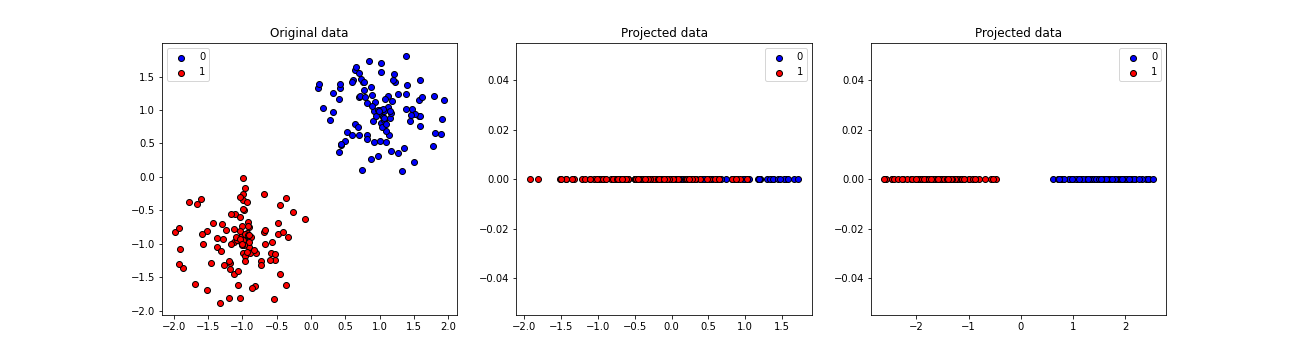
\includegraphics[width=\textwidth]{thesis/Figures/random_projections_example}
    \caption{Example of a dataset and two random projections of it. In the first projection, we can see
    that the points from the positive and the negative classes are almost totally overlapped, whereas in the
    second projection they are completely separable.}
    \label{fig:random_projections_example}
\end{figure}

\subsection{Random hyperplanes}

The second invariant that we propose is the random hyperplane. With it, we aim to create two partitions of
the original data: the samples that are on the right side of the hyperplane and the ones on the left, which
we will consider as the positive and the negative samples, respectively. Opposite to the previous invariant, which
produced a real value when applied to a point $x$, this one produces a discrete value $\set{0, 1}$ based on the
relative position of the point with respect to the normal vector of the hyperplane.
Figure \ref{fig:random_hyperplanes_example} shows an example of how this invariant works when applied to
an example dataset.

Formalizing the previous explanation, consider an arbitrary point from the sample $x_c \in \reals{d}$. Let
$n \sim \mathcal{N}(\mu, \Sigma)$ be the normal vector of the hyperplane that contains $x_c$, where the
multivariate normal distribution has mean $\mu \in \reals{d}$ and covariance matrix $\Sigma \in \reals{d \times d}$.
We can define the random hyperplane invariant as

\begin{equation}
    \label{eq:random_hyperplane_invariant}
    \psi_{r.h.}(x) =
    \begin{cases}
        1 & \text{if $(x - x_c)n \geq 0$ }\\
        0 & \text{otherwise}
    \end{cases}
\end{equation}

Considering the previous expression, we can clearly see that this invariant will yield a vector of zeroes
and ones when applied to a dataset. If we also take into account expression \eqref{eq:invariant_approximation},
we can deduce that this invariant will try to preserve the proportion of positive samples that fall on the right
side of the hyperplane. Consequently, we can see that this is a variation of the zeroth order invariant.
The main difference is that we are now trying to preserve the proportion of positive elements in a subspace
of the original space (the subspace formed by the samples that are on the same side as the normal vector of the
hyperplane), instead of trying to preserve it in the whole space.

\begin{figure}[h]
    \centering
    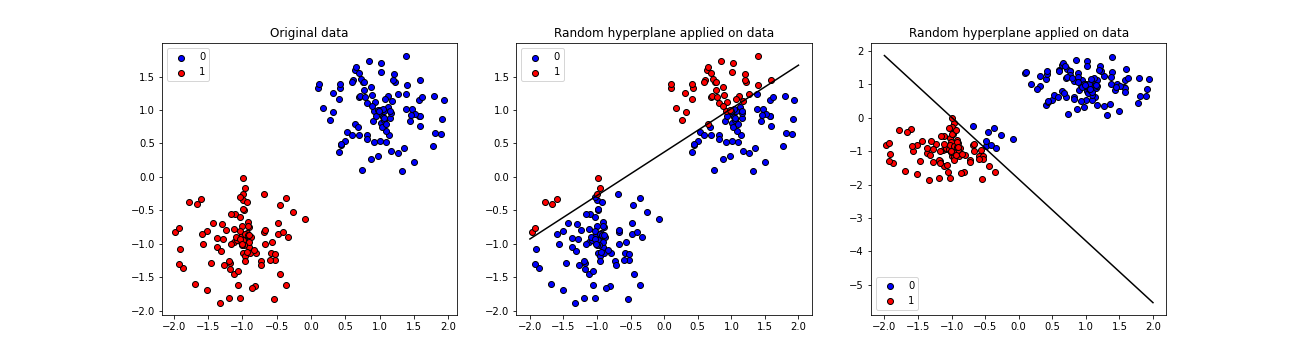
\includegraphics[width=\textwidth]{thesis/Figures/random_hyperplanes_example.png}
    \caption{Example of the hyperplanes invariant. In the left image, we can see the original data. In
    the middle and right images we can see two hyperplanes that divide the data in elements which are
    on the right and the left of the hyperplane, labeled as 1 and 0 respectively. Note that these
    new labels do not necessarily match the original ones.}
    \label{fig:random_hyperplanes_example}
\end{figure}

\section{Extending the LUSI paradigm to multiclass problems}

As we have seen up until now, this learning paradigm can be easily applied to binary classification problems
and solve them. Nevertheless, note that the invariants are defined specifically for just one of the classes. This ignores the invariant information that could be gathered by considering the other class. Moreover, in the most general setting of multiclass classification, the algorithm has to be extended. So, instead of restraining ourselves to a particular kind of problems, it seems reasonable trying to extend
LUSI to multiclass problems so that we have a wider application scope.

One framework that can be used to easily deal with this kind of problems is Error Correcting Output Codes (ECOC),
introduced by \cite{DietrichBakiri1995}. We can use it to treat multiclass classification problems as if they
were binary. For each one of the $N_c$ classes we create a codeword of length $n$. These codewords can be arranged as
the rows of a matrix called the \emph{coding matrix} $M \in \set{0, 1}^{N_c \times n}$. Each column of the matrix
is treated as an individual binary classification problem and a binary classifier is trained for each one of these
problems using the corresponding encoding (the columns).

An example of this can be seen in tables \ref{tab:ecoc_example_identity} and \ref{tab:ecoc_example_complex},
which show two different coding matrices for the same 5-class classification problem. The first one encodes the
problem as five one-against-all problems, which means that in each problem there will be only one class that can be
considered the positive one. In the second matrix, we can appreciate that some classes are encoded more than
once as the positive class.

\begin{table}[H]
\centering
\begin{tabular}{c|ccccc}
            & $h_1$ & $h_2$ & $h_3$ & $h_4$ & $h_5$ \\ \hline
\textbf{C1} & 1     & 0     & 0     & 0     & 0     \\
\textbf{C2} & 0     & 1     & 0     & 0     & 0     \\
\textbf{C3} & 0     & 0     & 1     & 0     & 0     \\
\textbf{C4} & 0     & 0     & 0     & 1     & 0     \\
\textbf{C5} & 0     & 0     & 0     & 0     & 1    
\end{tabular}%
\caption{Coding matrix for a multiclass classification problem with 5 classes and codewords of length $n=5$.
This matrix defines a special coding called one-against-all.}
\label{tab:ecoc_example_identity}
\end{table}


\begin{table}[H]
\centering
\begin{tabular}{c|ccccc}
            & $h_1$ & $h_2$ & $h_3$ & $h_4$ & $h_5$ \\ \hline
\textbf{C1} & 1     & 1     & 1     & 0     & 0     \\
\textbf{C2} & 0     & 1     & 1     & 0     & 1     \\
\textbf{C3} & 1     & 0     & 0     & 1     & 0     \\
\textbf{C4} & 0     & 1     & 0     & 1     & 0     \\
\textbf{C5} & 0     & 0     & 1     & 0     & 1    
\end{tabular}
\caption{Another coding matrix for the same 5-class classification problem.}
\label{tab:ecoc_example_complex}
\end{table}

Suppose that we have already trained a binary classifier for each one of the problems and we want to
predict the class for a given data point $x$. Let us denote $f(x) = (f_1(x), \dots, f_n(x))$ the
vector containing the predictions for each one of the problems. In order to obtain the corresponding output
class, we would need to decode this vector of predictions using the coding matrix that we have defined
for the problem. This is usually done by using some kind of distance metric and selecting the class with
the closest codeword according to the selected metric.

There are many distance metrics that we could use: Hamming distance, Euclidean distance, etc. In this
particular case, we have considered the Euclidean distance, which we will denote as $d_E$ and is computed
as $d_e(x, x') = \norm{x - x'}_2$. Let $M_r \in M$ be the $r$-th row of the coding matrix
We can express the predicted class $\hat{y}$ as

\begin{equation}
    \label{eq:ecoc_decoding}
    \hat{y} = \argmin_r d_E(M_r, f(x))
\end{equation}

Thus, the predicted class will be the one associated to the row that is closest to the vector of predictions.
Something important that we have to consider is that the binary classifiers for each problem should return the
probability $P(y=1 | x)$ rather than the actual label, which means that no threshold should be applied
during the prediction stage. This is because using the label directly might cause some errors when computing
the closest codeword. For example, consider the coding matrix defined in \ref{tab:ecoc_example_identity} and that
we are given a vector of predictions $(1, 1, 0, 0, 0)$ whose associated vector of probabilities is
$(0.8, 0.55, 0.4, 0.1, 0.25)$. If we consider the binary vector of predictions, then both class 1 and
class 2 are the closest ones, which will lead to randomly selecting among them and to a potential missclassification
since class 1 is the most probable 1. However, if we consider the vector of probabilities, then the closest
class in this case will be class 1, which is indeed the most probable one.

In consequence, in order to extend LUSI to multiclass classification problems we have to follow these steps:

\begin{enumerate}[label=\textbf{Step \arabic*:}]
    \item Create the coding matrix $M$ of size $N_c \times n$.
    \item Use the columns of $M$ to generate new binary labels for each one of the $n$ binary classification problems.
    \item Train $n$ binary classifiers that use LUSI with the previously generated binary labels.
    \item Given an input data point $x$, predict the vector of probabilities using the previous binary classifiers.
    \item Select the output class using expression \eqref{eq:ecoc_decoding}.
\end{enumerate}

\chapter{Experimentation and results}
\label{Chapter4}

After having explained the necessary theoretical background and presented the proposals
of this work, it is time that we put them into action to see how they perform. First, we are going
to test our proposals on some toy datasets in order to better understand them. After that, we are going
to try the proposed invariants as well as the multiclass extension with ECOC on real data to see how
well they perform when comparing them to the original invariants proposed in \cite{Vapnik2019}.

\section{Experimenting with toy problems}

In this section we will perform a set of simple experiments with some toy datasets. In this case, we have
considered the circles and moons datasets, which can be seen in figure \ref{fig:toy_datasets}. Both of
these problems are available in \texttt{scikit-learn}, which means that we will be able to easily generate
our custom datasets with the available functions. When experimenting with these problems we aim to:

\begin{itemize}
    \item Compare the original invariants with the ones that have been proposed in this work.
    \item Compare the original version of the LUSI algorithm with the ECOC version to see if there is
    any significant difference in a binary setting.
    \item Discover whether some types of invariants are more likely to be selected when considering all types
    of invariants.
\end{itemize}

\begin{figure}[H]
    \centering
    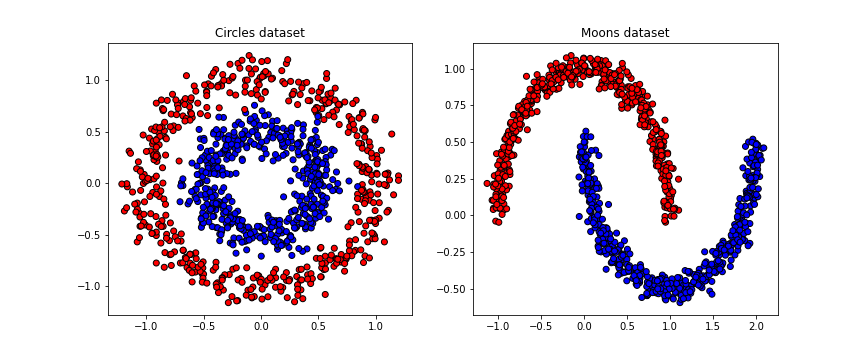
\includegraphics[width=\textwidth]{thesis/Figures/toy_datasets.png}
    \caption{Toy datasets used in the experimentation.}
    \label{fig:toy_datasets}
\end{figure}

\subsection{Experimental settings}

For this experimentation, we have generated one dataset for each problem with a fixed seed. The experimental
parameter settings for each type of problem can be seen in table \ref{tab:toy_problems_experiments}. In an experiment,
we split the data in training and test, keeping 10\% of the data in the training partition and the reamining
90\% in the test partition. We have performed these experiments using Vapnik's invariants and the ones
that we have proposed. As for Vapnik's invariants, we have considered the zeroth and first order invariants, which are

\[
    \psi_0(x) = 1,\quad \psi_1(x) = x_1,\quad \psi_2(x) = x_2
\]

\begin{table}[h]
\centering
\begin{tabular}{llr}
\textbf{Problem} & \textbf{Parameter}  & \textbf{Value} \\ \hline
Circles          & \texttt{n\_samples} & 1000           \\
                 & \texttt{noise}      & 0.1            \\
                 & \texttt{factor}     & 0.5            \\
Moons            & \texttt{n\_samples} & 1000           \\
                 & \texttt{noise}      & 0.05          
\end{tabular}
\caption{Parameter settings of the toy problems.}
\label{tab:toy_problems_experiments}
\end{table}

\subsection{Comparing the different invariant types and versions of LUSI}

In order to compare the two versions of the LUSI algorithm and the different invariants
we have trained a model for each version of LUSI and each invariant type on both problems with a fixed
initial random state. We have visualized the decision boundaries in each case in order to see if there is any
significant difference between them. Additionally, for the LUSI version we have reported the mean number of selected
invariants of each type by repeating the experiment with 10 different initial states. We have limited the
maximum number of invariants of each model to 3 because even though we can generate infinite new random
invariants, we cannot do the same with the original invariants.

Figures \ref{fig:circles_decision_boundary} and \ref{fig:moons_decision_boundary} show the decision
boundaries generated by the original version of the LUSI algorithm whereas figures
\ref{fig:circles_decision_boundary_ecoc} and \ref{fig:moons_decision_boundary_ecoc} display the decision
boundaries of the ECOC version. For the circles problem, we can see that all invariants produce
very similar decision boundaries. In the case of ECOC version, this decision boundary seems to be much
closer to the points of the blue class than in the case of the original algorithm, where the decision boundary
is a bit wider. As for the moons problem, we can observe that the decision boundary is not perfect
in any of the versions of the algorithm since some points fall into the region of the opposite class,
probably caused by to the geometric shape of the both classes. For this problem, the decision boundary seems
to be more accurate using the original algorithm. This is especially true in the case of the random hyperplanes,
where the decision boundary is better adjusted in the case of the original algorithm, whereas it seems that it
has been overfitted when using the ECOC algorithm because we can observe some ``decision islands'' for the blue
class. Overall, it seems that Vapnik's invariants and the random projections produce very similar results
regardless of which version of the algorithm is applied. Hence, if we use any of these two invariants, we
could apply any version of the algorithm and get similar results in a binary classification problem. In the
case of the random hyperplanes, there would be some difference between the results obtained with each version
of the algorithm. As we have seen, depending on the problem, we could get similar results to the ones obtained
using the other two types of invariants.

The idea that Vapnik's invariants and the random projections are similar can be further explored. Figure
\ref{fig:toys_small_num_selected_invariants} show how many invariants have been selected for each problem
on average. We can observe that the mean number of selected invariants is the same for Vapnik's invariants
and the random projections, whereas the number of selected invariants is equal to the maximum number of
invariants in the case of the random hyperplanes. Thus, it seems that the number of invariants that can be
chosen when using Vapnik's invariants and the random projections is limited by the number of dimensions of the
data, as selecting more does not provide any new information. In the case of the random hyperplanes, this is
generally not true as we could keep adding more invariants of this type. This might be caused by the
fact that there is a very large number of hyperplanes that separate the data in two partitions and that
can be used to preserve the proportion of elements that fall on the right side of the hyperplane.
Because of this, many invariants of this type can be selected.

\subsection{Exploring the bias towards certain types of invariants}

Now, we would like to study the scenario in which all types of invariants are considered to see if there is
any kind of bias towards particular types of invariants. For this purpose, we have run a similar experiment to
the previous one using the original version of the LUSI algorithm. We have fit 10 models on both problems
using different random states and setting the maximum number of invariants to 50. In each experiment, the
model could choose among all of the invariant types. For each run, we have computed how many invariants of
each type were selected.

A summary of the results can be seen in figure \ref{fig:toys_mean_num_selected}, where the number of
selected invariants has been averaged for each problem. We can see that the models have not selected any of
Vapnik's invariants. On average, they have chosen 2 random projections per problem, which once again matches
the number of dimensions that these problems have. The models have selected 48 random hyperplanes on average
per problem, which gives more strength to the hypothesis that the number of hyperplane invariants that
can be selected is very large, potentially infinite. Because of this, we can see that when considering
all types of invariants at the same time, it is more likely that the hyperplanes invariant will be selected
because it can contribute with more information.

\section{Experimentation on real data}

After testing our proposals on some toy problems and comparing them to the original work, it is time that we
put them into action on real problems. With this experimentation we want to study the quality of the
new invariants compared to Vapnik's proposals to see if we have achieved our goal of creating general purpose
invariants that can be applied to multiple problems and that allow us to obtain quality results. In this section,
we are going to present the experiments that we have performed as well as the obtained results.

\begin{figure}[H]
    \centering
    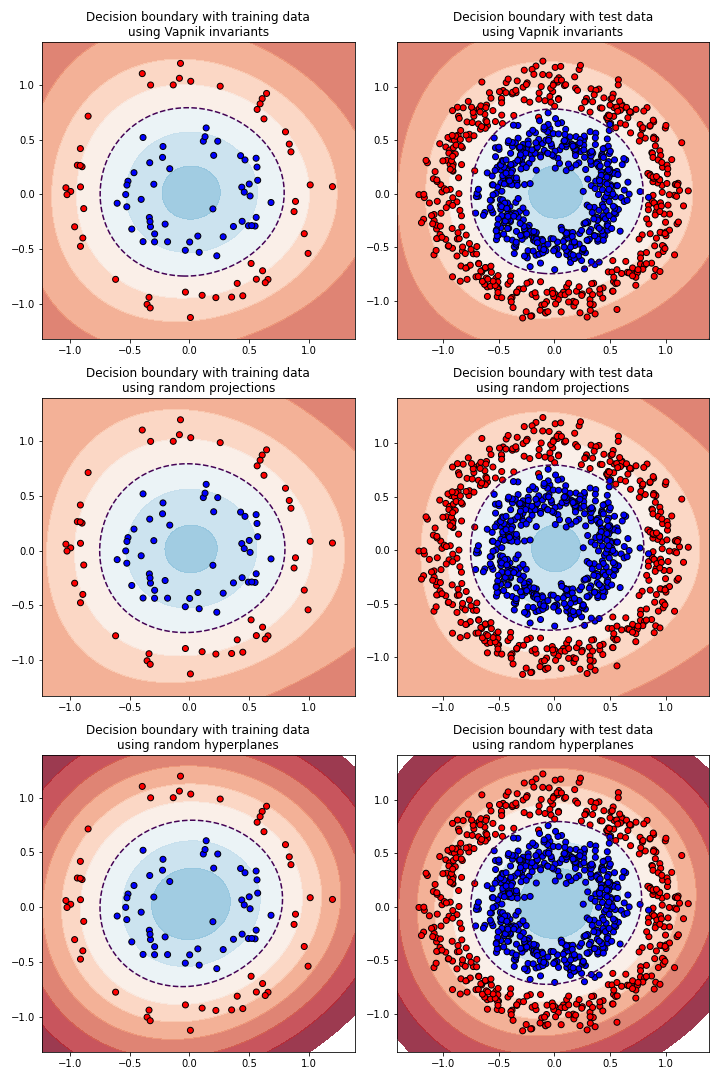
\includegraphics[width=\textwidth]{thesis/Figures/circles_decision_boundaries.png}
    \caption{Decision boundaries in the circles problem using the original LUSI algorithm with each type of
    invariant on the training and test sets.}
    \label{fig:circles_decision_boundary}
\end{figure}

\begin{figure}[H]
    \centering
    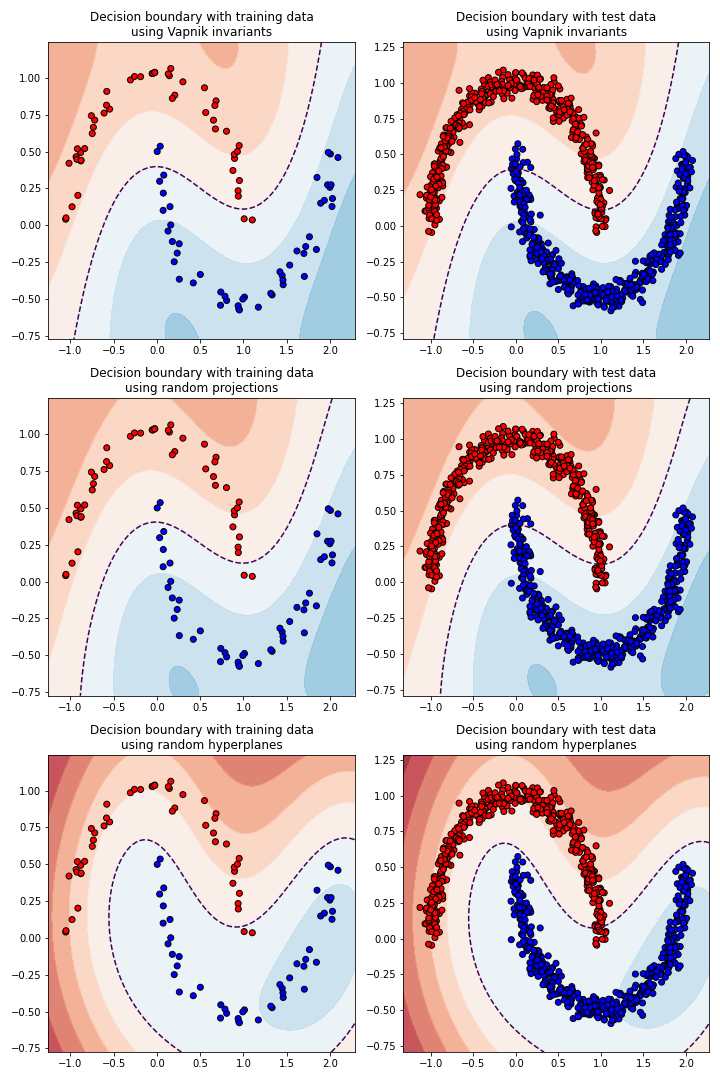
\includegraphics[width=\textwidth]{thesis/Figures/moons_decision_boundaries.png}
    \caption{Decision boundaries in the moons problem using the original LUSI algorithm with each type of
    invariant on the training and test sets.}
    \label{fig:moons_decision_boundary}
\end{figure}

\begin{figure}[H]
    \centering
    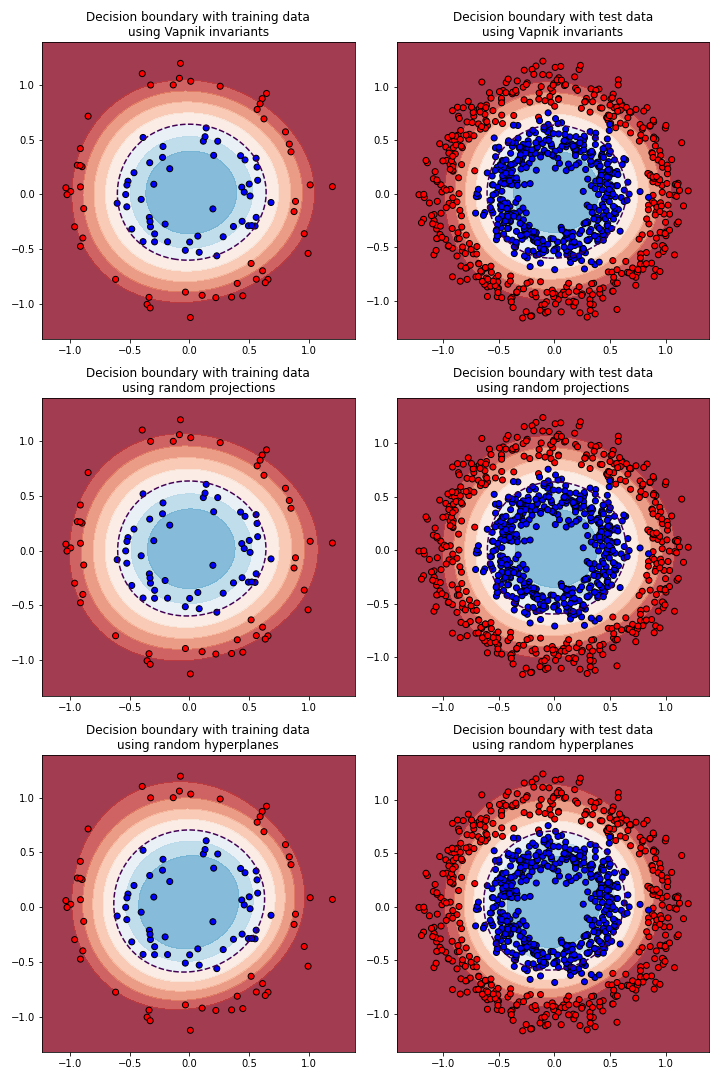
\includegraphics[width=\textwidth]{thesis/Figures/circles_decision_boundaries_ecoc.png}
    \caption{Decision boundaries in the circles problem using the ECOC version of the LUSI algorithm with each type
    of invariant on the training and test sets.}
    \label{fig:circles_decision_boundary_ecoc}
\end{figure}

\begin{figure}[H]
    \centering
    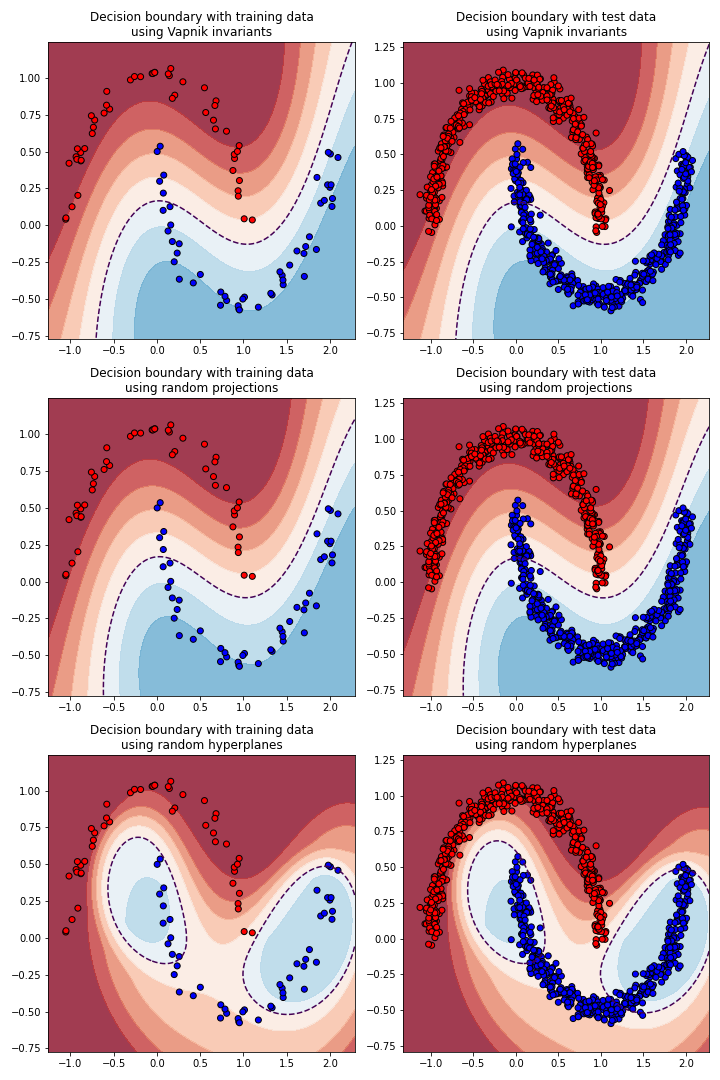
\includegraphics[width=\textwidth]{thesis/Figures/moons_decision_boundaries_ecoc.png}
    \caption{Decision boundaries in the moons problem using the ECOC version of the LUSI algorithm with each type
    of invariant on the training and test sets.}
    \label{fig:moons_decision_boundary_ecoc}
\end{figure}

\begin{figure}[H]
    \centering
    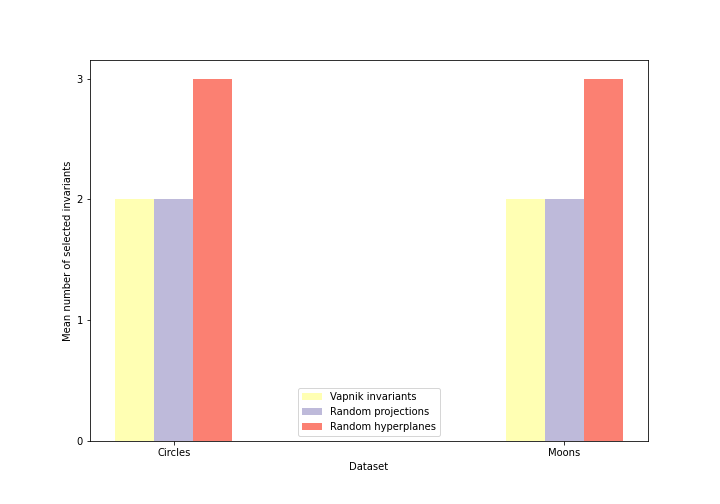
\includegraphics[width=0.8\textwidth]{thesis/Figures/num_selected_invariants.png}
    \caption{Mean number of selected invariants per problem. The maximum number of invariants was set to 3.}
    \label{fig:toys_small_num_selected_invariants}
\end{figure}

\begin{figure}[H]
    \centering
    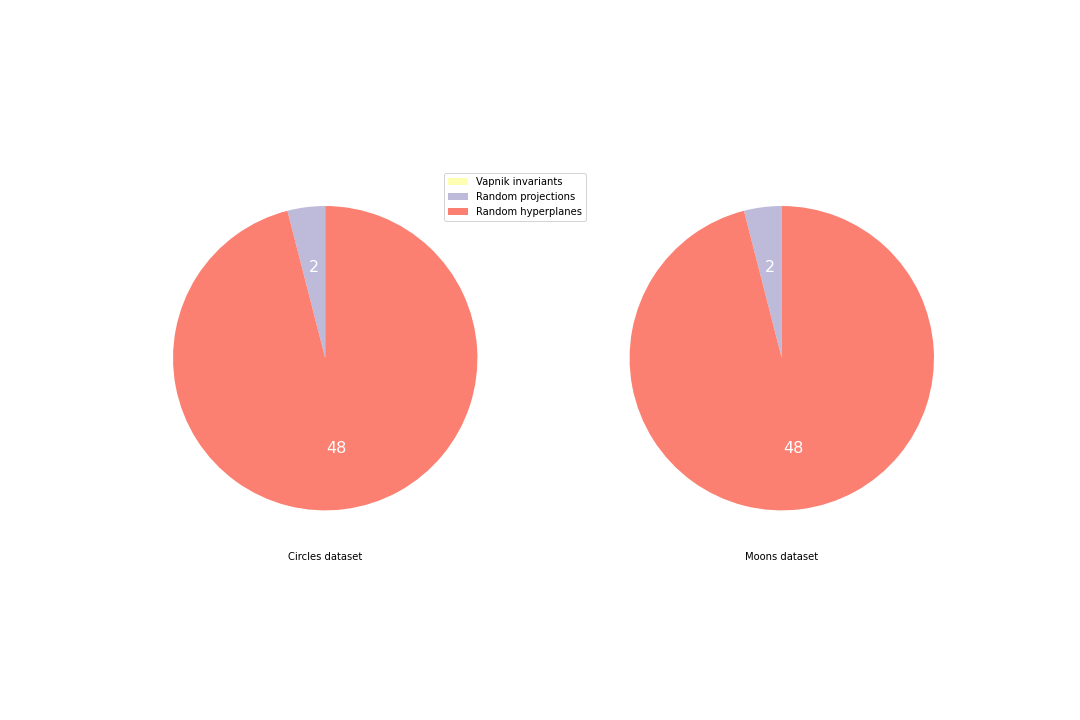
\includegraphics[width=\textwidth]{thesis/Figures/mean_num_selected.png}
    \caption{Mean number of selected invariants when the maximum number of invariants is 50 and the three types of
    invariants are considered simultaneously.}
    \label{fig:toys_mean_num_selected}
\end{figure}


\subsection{Experimental settings}

First and foremost, we need to discuss what datasets we are going to use in the experimentation, what
will be compared and how the experiments will be performed.

As for the data, we are going to use five datasets from the UCI repository (\cite{UCIRepository}). Originally, we
planed on using more datasets, but due to strong time restrictions and the fact that each experiment took from a couple
of hours up to a couple of days it did not seem worthwhile increasing the number of datasets. The selected datasets
along with some basic information about them can be found in table \ref{tab:problems_description}. As we can see, all
of them are multiclass classification problems, which means that we must use the ECOC-based extension that we have
proposed in this work. We applied some preprocessing to the datasets before using them in our experiments, like
transforming the categorical values using hashing and transforming the classes to numerical values so that we
could more easily create the encoding matrices and apply the posterior decoding step.

\begin{table}[H]
\centering
\begin{tabular}{lrrr}
\textbf{Problem} & \textbf{Num. examples} & \textbf{Attributes} & \textbf{Classes} \\ \hline
Balance Scale    & 625                    & 4                   & 3                \\
Ecoli            & 336                    & 8                   & 8                \\
Glass            & 214                    & 9                   & 7(6)\tablefootnote{According to the dataset's documentation, there are 7 classes. However, there is one that does not have any elements. Therefore, the actual number of classes for this problem is 6.}                \\
Iris             & 150                    & 4                   & 3                \\
Yeast            & 1484                   & 8                   & 10              
\end{tabular}
\caption{Information of the datasets used in the experimentation.}
\label{tab:problems_description}
\end{table}

In these experiments, we will be comparing four different versions of LUSI using different types of invariants:
\begin{enumerate*}[label=(\roman*)]
    \item a baseline version with no invariants,
    \item Vapnik's invariants (zeroth and first order invariants),
    \item random projections and
    \item random hyperplanes.
\end{enumerate*}

In order to compare the different models, we have designed an experimentation methodology that we will briefly
describe. We are going to create three different stratified partitions of each dataset using different seeds.
In these partitions we are going to keep 80\% of the data for training and the remaining 20\% will be used to
test the models. For each training partition, we are going to create three different stratified subsamples of it,
keeping 100\%, 50\% and 10\% of the data. Using each one of these subsamples, we are going to perform three grid
searches using 3-fold cross validation over different combinations of hyperparameters for each one of the models,
finding the best possible combination of hyperparameters in each case. Finally, we are going to evaluate these
models using the test set from the corresponding partition and obtain a accuracy for that particular scenario.
We are using the same test partition to evaluate the different models so that we can have a common ground that allows
us to fairly compare the different types of invariants. A general overview of this experimentation methodology
can be seen in figure \ref{fig:experimentation_setup}, where an example is shown using the random projections
invariant.

Finally, we need to clarify which hyperparameters we are going to be fine-tuning. For this experimentation and due
to the previously mentioned time restriction as well as the hefty amount of hyperparameter combinations for each
model, we have restricted ourselves to performing the grid search on the following hyperparameters:

\begin{itemize}
    \item The maximum number of invariants that can be selected.
    \item The value of $\delta$ used in the invariants selection.
    \item The value of $\gamma$ used when computing the kernel.
    \item The value of \texttt{C}, which is a regularization parameter that controls how much perturbation
    is applied to the product of the $V$ and $K$ matrices before computing the inverse so that it is not a
    singular matrix.
\end{itemize}

\begin{figure}[h]
    \centering
    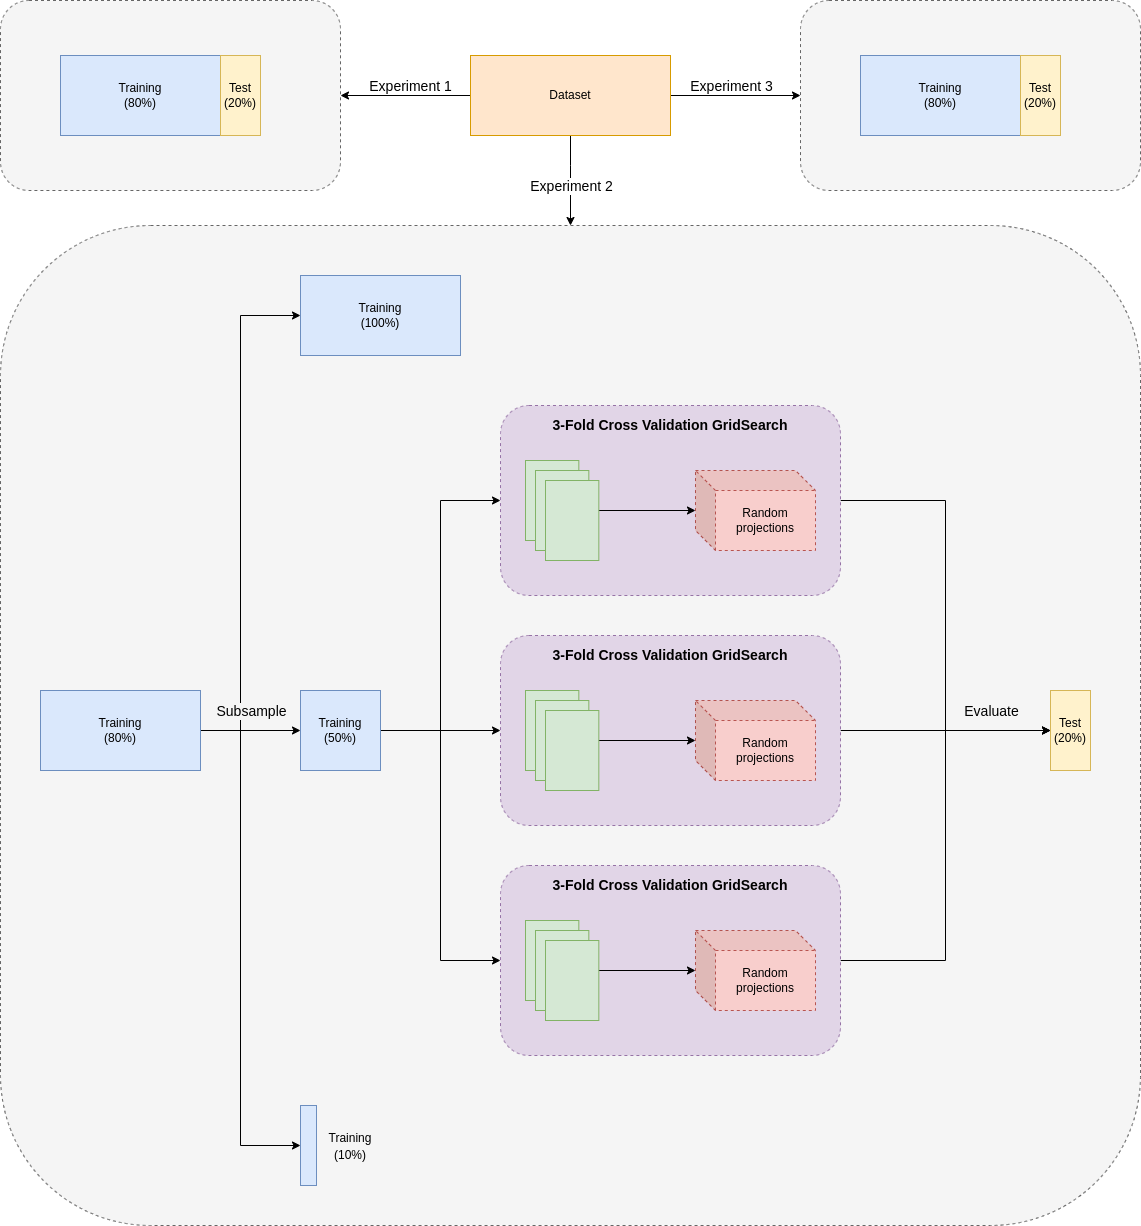
\includegraphics[width=\textwidth]{thesis/Figures/experimentation_scheme.drawio.png}
    \caption{Overview of the experimentation methodology. In this example, the grid search is only applied to
    the random projections model for a subsample of 50\% of the training partition, although in a real scenario
    it would be applied to each training subsample and to each type of model. Note that all models are evaluated using
    the same test partition.}
    \label{fig:experimentation_setup}
\end{figure}

\subsection{Results}

Let us now analyze the results that we have obtained from the experimentation. Table \ref{tab:results_accuracies_errors}
contains the mean accuracies and standard deviations for each dataset considering the different invariant types
and training subsample sizes. We have only reported the mean accuracies achieved when using a subsample
of 100\% and 10\% of the training partitions, as they represent two extremes of the learning problem: one in which
there is a lot of available training data, and one where this data is scarce.

We can observe that the baseline model with no invariants almost completely outperforms the rest of the
models which use some kind of invariants on both training sizes. Also, it is the one that has the
least variation in the results. In second place we find the original invariants proposed by Vapnik, which
offer good results overall, although a model that uses no invariants is capable of achieving better results.
The random projections follow quite closely Vapnik's invariants, offering average results that are a bit worse
than the original invariants. However, they are capable of achieving better results than Vapnik's invariants in
the Balance Scale dataset using a big training size and in the Glass dataset when considering a small training
dataset. The large deviation in the Iris dataset in the small problem is really curious, probably caused by a
bad random seed. Finally, the random hyperplanes come in last place, offering the worst results in almost all
problems irregardless of the training size.

One possible explanation for the poor results obtained by the random invariants may be that the random
seeds that we have chosen are quite bad. Because these invariants heavily rely on stochastic processes,
a bad initialization can greatly worsen the results. Thus, we can try to repeat these
experiments with more carefully selected random seeds or by increasing the pool of initial seeds, which
would mean that we would have to run more experiments, which as we have already mentioned, takes a very long
time and computational resources.

This randomness also affects the variation of the results. As we can clearly see, the models that use the
random invariants have larger standard deviations. Because the model that uses no invariants has no
need to select invariants and the one that uses Vapnik's proposed invariants does not have to generate new
invariants, the training process becomes more deterministic, which reduces the overall variability of the results.

Another result that must be highlighted is the poor performance of the random hyperplanes. A possible
explanation of this might be that this invariant is a modification of the zeroth order invariant in
which the proportion of elements is only kept in a region of the original space. Although the idea seemed
interesting in the first place as we have potentially infinite hyperplanes that can separate the data in order
to keep different proportions of it, in practice it seems that preserving this kind of statistical information
might not be that useful as the models may be prone to overfitting, as we saw in the experimentation with the toy
problems.

\begin{table}[h]
\centering
\resizebox{\textwidth}{!} &
  10\% &
  \multicolumn{1}{c|}{100\%} &
  10\% &
  \multicolumn{1}{c|}{100\%} &
  10\% &
  \multicolumn{1}{c|}{100\%} &
  10\% \\ \hline
\multicolumn{1}{|c|}{Balance Scale} &
  \multicolumn{1}{c|}{$91.47 \pm 0.38\%$} &
  $88.80 \pm 1.73\%$ &
  \multicolumn{1}{c|}{$91.47 \pm 0.38\%$} &
  $87.73 \pm 2.10\%$ &
  \multicolumn{1}{c|}{$91.73 \pm 0.38\%$} &
  $83.73 \pm 7.17\%$ &
  \multicolumn{1}{c|}{$90.13 \pm 1.51\%$} &
  $76.00 \pm 12.77\%$ \\ \hline
\multicolumn{1}{|c|}{Ecoli} &
  \multicolumn{1}{c|}{$85.29 \pm 2.08\%$} &
  $71.57 \pm 1.39\%$ &
  \multicolumn{1}{c|}{$85.29 \pm 1.20\%$} &
  $72.55 \pm 4.22\%$ &
  \multicolumn{1}{c|}{$84.15 \pm 2.05\%$} &
  $67.32 \pm 4.03\%$ &
  \multicolumn{1}{c|}{$75.98 \pm 6.28\%$} &
  $63.89 \pm 9.61\%$ \\ \hline
\multicolumn{1}{|c|}{Glass} &
  \multicolumn{1}{c|}{$72.87 \pm 7.91\%$} &
  $56.59 \pm 4.78\%$ &
  \multicolumn{1}{c|}{$72.87 \pm 7.91\%$} &
  $45.74 \pm 6.67\%$ &
  \multicolumn{1}{c|}{$72.09 \pm 7.44\%$} &
  $52.45 \pm 7.03\%$ &
  \multicolumn{1}{c|}{$71.06 \pm 7.60\%$} &
  $45.48 \pm 9.50\%$ \\ \hline
\multicolumn{1}{|c|}{Iris} &
  \multicolumn{1}{c|}{$96.67 \pm 0.00\%$} &
  $93.33 \pm 2.72\%$ &
  \multicolumn{1}{c|}{$95.56 \pm 1.57\%$} &
  $90.00 \pm 4.71\%$ &
  \multicolumn{1}{c|}{$95.19 \pm 1.66\%$} &
  $77.78 \pm 22.93\%$ &
  \multicolumn{1}{c|}{$88.52 \pm 11.56\%$} &
  $84.81 \pm 9.04\%$ \\ \hline
\multicolumn{1}{|c|}{Yeast} &
  \multicolumn{1}{c|}{$53.76 \pm 1.04\%$} &
  $47.92 \pm 2.08\%$ &
  \multicolumn{1}{c|}{$53.87 \pm 1.20\%$} &
  $47.92 \pm 2.14\%$ &
  \multicolumn{1}{c|}{$52.53 \pm 5.44\%$} &
  $45.68 \pm 4.60\%$ &
  \multicolumn{1}{c|}{$50.39 \pm 5.33\%$} &
  $37.82 \pm 7.92\%$ \\ \hline
\end{tabular}%
}
\caption{Mean accuracy and standard deviation for each type of invariant in each problem considering
the results for subsamples of 100\% and 10\% of the training data. The results are expressed as percentages.}
\label{tab:results_accuracies_errors}
\end{table}

We can delve into the previous results by comparing how many times each model obtains a better, worse
or the same accuracy as the rest of the models for the same experiment. This information has been
condensed in figure \ref{fig:invariants_performance}, where we can see the performance of the
different models across all experiments.

As we can observe, the model with no invariants is capable of achieving more times greater accuracies than
the rest of the models irregardless of the training size. When compared to the model that uses Vapnik's invariants,
we can see that they achieve the same accuracy in a lot of experiments (approximately 50\% of the times). This
model offers worse results in only a couple of experiments, which are less than 20\% of the times. Something similar
happens when we compare it to the random projections, although the results are a bit more favorable for the model
with no invariants in this case. When comparing it to the random hyperplanes, we can see that the latter one
is totally outmatched.

If we compare now Vapnik's invariants to the random projections, we can see that they achieve very similar
results overall, although they are more favorable in the case of Vapnik's invariants. When comparing
these invariants with small training sizes, we can see that the difference between them is less significant.
Hence, as we saw in the previous experimentation and in this one, we can state that these types of invariants are
very similar. Probably, this is due to the fact that most of Vapnik's invariants are first order invariants,
and the random projections are a variation of this type of invariant. With them, we can preserve the centroid of
each class, which is an interesting information that should be kept when learning the bets approximation of the
target function.

Finally, to no one's surprise, the random hyperplanes are the ones that perform the worst when compared to the
rest of the models, as it is the invariant type that gets beaten the most frequently. This might be because the
information provided by this variation of the zeroth order invariant is not as relevant as the one provided by
the original zeroth order invariant or higher order invariants. Hence, its usefulness seems questionable even
when a model that uses no invariants is capable of outperforming a model that uses this kind
of invariant by far.

\begin{figure}[ht]
    \centering
    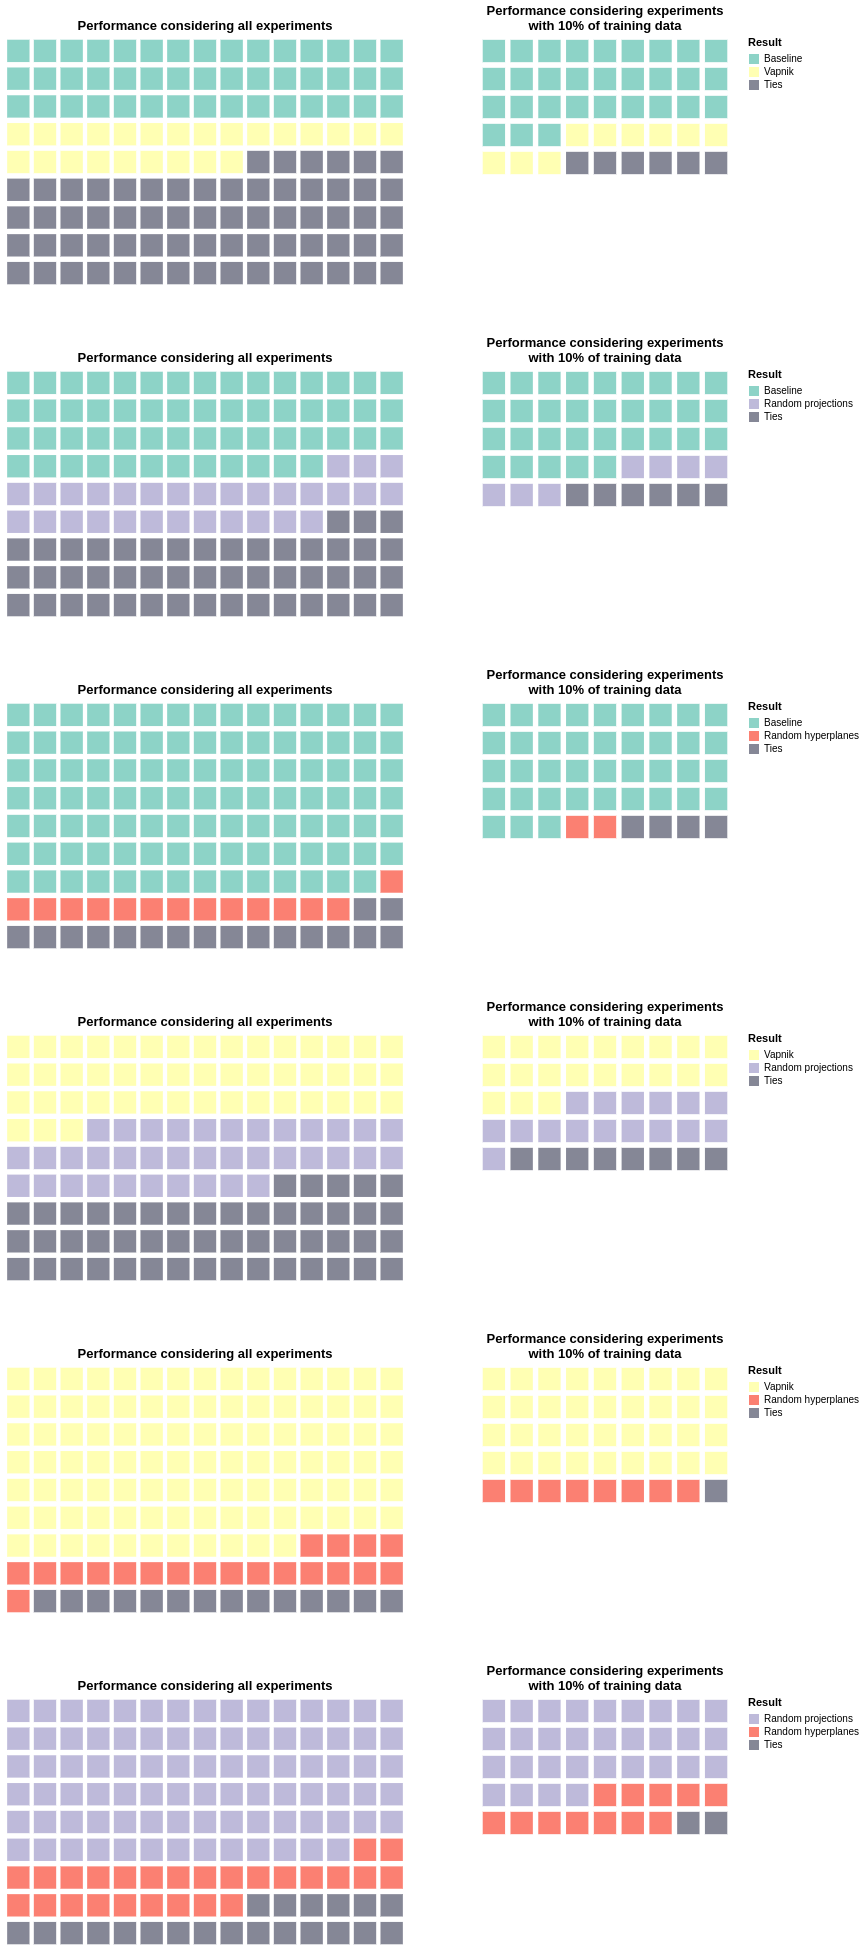
\includegraphics[width=0.65\textwidth]{thesis/Figures/invariants_performance.png}
    \caption{Waffle charts showing the number of times that each model achieves a better, worse or the same
    accuracy when compared to the accuracy achieved by another model in the same experiment, aggregated
    across all datasets. Left column shows the results obtained when the training size is disregarded.
    The right one shows the results only when considering the experiments where 10\% of the training partition
    is used.}
    \label{fig:invariants_performance}
\end{figure} 
% Chapter Template

\chapter{Experimentation and results} % Main chapter title
\label{Chapter4}

\label{ChapterX} % Change X to a consecutive number; for referencing this chapter elsewhere, use \ref{ChapterX}

\section{Experimenting with toy problems}

\section{Experimentation on real data}

\subsection{Methodology}

\subsection{Results}


%----------------------------------------------------------------------------------------
%	THESIS CONTENT - APPENDICES
%----------------------------------------------------------------------------------------

% \appendix % Cue to tell LaTeX that the following "chapters" are Appendices

% Include the appendices of the thesis as separate files from the Appendices folder
% Uncomment the lines as you write the Appendices

% % Appendix A

\chapter{Frequently Asked Questions} % Main appendix title

\label{AppendixA} % For referencing this appendix elsewhere, use \ref{AppendixA}

\section{How do I change the colors of links?}

The color of links can be changed to your liking using:

{\small\verb!\hypersetup{urlcolor=red}!}, or

{\small\verb!\hypersetup{citecolor=green}!}, or

{\small\verb!\hypersetup{allcolor=blue}!}.

\noindent If you want to completely hide the links, you can use:

{\small\verb!\hypersetup{allcolors=.}!}, or even better: 

{\small\verb!\hypersetup{hidelinks}!}.

\noindent If you want to have obvious links in the PDF but not the printed text, use:

{\small\verb!\hypersetup{colorlinks=false}!}.

%\include{Appendices/AppendixB}
%\include{Appendices/AppendixC}

%----------------------------------------------------------------------------------------
%	BIBLIOGRAPHY
%----------------------------------------------------------------------------------------

\printbibliography[heading=bibintoc]

%----------------------------------------------------------------------------------------

\end{document}  
